\documentclass[10pt]{article}
\usepackage[a4paper,margin=.72in,headheight=15pt]{geometry}
\usepackage[T1]{fontenc}\usepackage[utf8]{inputenc}\usepackage{lmodern,microtype,amsmath,amssymb,graphicx,xcolor,booktabs,tabularx,hyperref,fancyhdr}
\definecolor{ink}{HTML}{153F50}\definecolor{accent}{HTML}{0072B2}
\setlength{\parindent}{0pt}\setlength{\parskip}{7pt}\setlength{\emergencystretch}{3em}
\hypersetup{colorlinks=true,urlcolor=accent}
\pagestyle{fancy}\fancyhf{}\fancyhead[L]{\small\color{ink}GLOVER | INDEPENDENT RESEARCH WHITE PAPER}\fancyhead[R]{\small 2026}\fancyfoot[C]{\thepage}
\begin{document}

{\small\color{accent}Research argument}\par
{\LARGE\bfseries\color{ink}Magnum Quantreleviathone}\par\vspace{7pt}
Michael Emanuel Glover\par Developed in dialogue with Codex | 4 October 2026\par\vspace{8pt}
Smaller representations, quantum fluctuations, and the limits of an ending. By Michael Emanuel Glover, developed in dialogue with Codex. This is a mathematical research note with a reproducible classical computation; the first-person framing expresses the author's proposed research direction.\par
I want to investigate quantum behavior at home, using the computer I already possess. My starting question is not whether a laptop becomes a physical quantum processor. It is whether an enormous state can sometimes have a small, exact description. In an important family of examples, the answer is yes. The research opportunity is to identify the structure before allocating the space.\par
The title names a leviathan of possibilities. Its mathematical task is modest and precise: prepare a family of entangled states, prove a compact description, and check the description against dense simulation. Its philosophical task is to distinguish a formal ending from an ending in nature. Neither a successful simulation nor the phrase "it is finished" proves that the universe has a terminating condition.\par
An axiom specifies this model. A theorem follows within it. A numerical check exercises an implementation. A physical experiment tests the model against observations. These are related activities with different evidential roles. This note claims the first three for the circuit below; it does not report a quantum-hardware experiment.\par
\clearpage
{\small\color{accent}Research argument}\par
{\LARGE\bfseries\color{ink}Axioms and an exact family}\par\vspace{7pt}
A1: an n-qubit pure state is a normalized vector in a complex Hilbert space of dimension two to the n. A2: closed-system gates in this model are unitary linear maps. A3: computational-basis measurement probabilities are squared amplitude magnitudes. These are modeling postulates of finite-dimensional quantum mechanics, not a derivation of all physics.\par
Define H on a single qubit by H|0>=(|0>+|1>)/sqrt(2) and H|1>=(|0>-|1>)/sqrt(2). Define controlled NOT as flipping a target bit precisely when its control bit is one. Start with every qubit zero, apply H to qubit zero, and then apply controlled NOT from that qubit to each remaining qubit.\par
Theorem: the resulting state is GHZ\_n. Proof: H produces two branches with equal amplitudes. In the zero-control branch every target remains zero. In the one-control branch each successive target becomes one. Induction on the number of targets gives the displayed state. The two basis states are orthogonal, so its squared norm is one. A3 gives equal measurement probabilities to the two outcomes and zero to every other outcome.\par
The description contains a qubit count, a gate pattern, and two amplitudes. For this family it avoids listing exponentially many zeros. The proof depends on the specific circuit; it is not a compression theorem for arbitrary quantum states.\par
\[\mathcal H_n=(\mathbb C^2)^{\otimes n},\qquad\sum_x |a_x|^2=1.\]
\[|\mathrm{GHZ}_n\rangle=\frac{|0\rangle^{\otimes n}+|1\rangle^{\otimes n}}{\sqrt2}.\]
\clearpage
{\small\color{accent}Research argument}\par
{\LARGE\bfseries\color{ink}Compute it: nineteen checked circuits}\par\vspace{7pt}
compute.py uses NumPy to implement the specified gates on dense complex128 arrays for every qubit count from two through twenty. It compares every final amplitude with the proven formula, checks normalization within tolerance, and checks that exactly two amplitudes are nonzero. This is a deterministic numerical validation, not a statistical trial or a benchmark against a quantum processor.\par
The twenty-qubit array occupies 16,777,216 bytes of amplitude storage. A sparse payload consisting of two complex128 amplitudes and two unsigned 64-bit indices occupies 48 bytes over the tested range. Python object overhead, allocator overhead, temporary arrays, executable storage, and the qubit-count metadata are excluded from that payload comparison. The code and JSON record these conventions explicitly.\par
Every tested amplitude matched the expected floating-point value exactly in this implementation; squared norms differed from one by at most ordinary floating-point rounding. Exact agreement between two floating-point paths is not an exact-arithmetic proof. The preceding induction supplies the mathematical result; the computation provides implementation evidence.\par
{\small\begin{tabularx}{\linewidth}{Xrr}\toprule
Qubits & Dense bytes & Sparse payload\\\midrule
2 & 64 & 48\\
10 & 16384 & 48\\
20 & 16777216 & 48\\
\bottomrule\end{tabularx}}\par
\begin{center}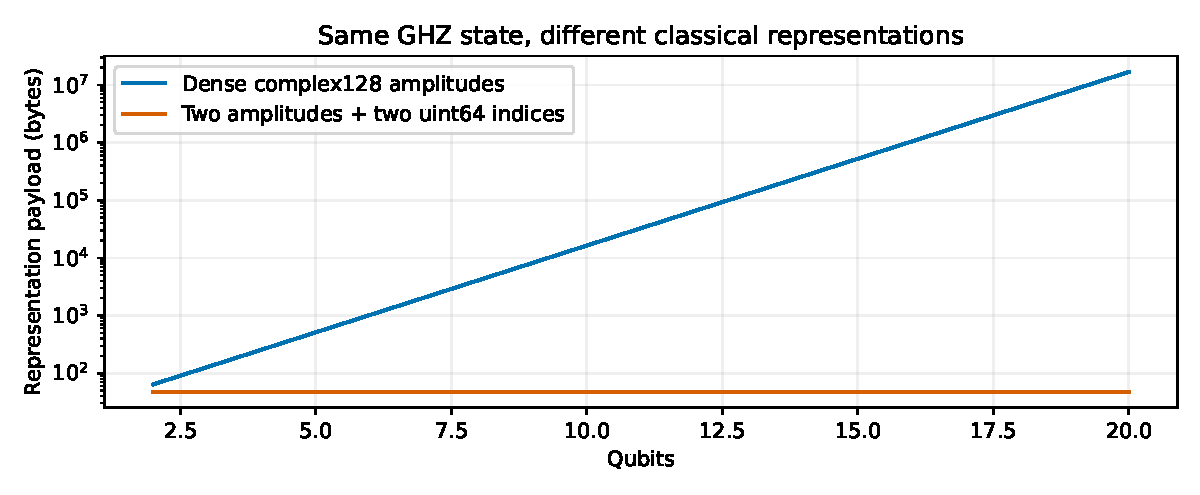
\includegraphics[width=.97\linewidth,height=.26\textheight,keepaspectratio]{figures/memory.pdf}\end{center}
{\footnotesize Computed array payloads for the GHZ family. The lower line describes a sparse payload, not the measured total RAM of the simulator.\par}
\clearpage
{\small\color{accent}Research argument}\par
{\LARGE\bfseries\color{ink}Fluctuations, perceptions, and conclusions}\par\vspace{7pt}
A quantum fluctuation can be described operationally as nonzero variance of an observable in a specified state. For a Hermitian observable A, the variance is its expected square minus the square of its expectation. Even a stationary state can have nonzero variance. This does not require a story of little objects spontaneously appearing and disappearing, nor does it imply that an entire universe has stopped evolving.\par
Quantum interactions do contribute to color vision: light is absorbed through molecular processes and produces signals that neural systems process. But a photon wavelength is not itself a complete account of a colorful experience. Illumination, receptors, context, and neural processing matter. The GHZ calculation here models none of those biological mechanisms and supplies no theory of consciousness.\par
Smaller is better when a representation preserves the queries we need while reducing actual resource costs. Sparse states, stabilizer descriptions, and suitable tensor-network structures offer different opportunities and limitations. Gottesman's stabilizer framework provides an established route for efficiently simulating a restricted class of circuits, including substantial entanglement. This broader result is cited, not proved here.\par
The conclusion is conditional and useful: this circuit family has a compact exact description, verified against nineteen dense simulations. A generic state need not have this sparsity; subsequent gates can destroy it. A rigorous next step is to expand the gate set, monitor representation growth, compare equal output queries, and report where compactness fails. No quantum advantage, new physical law, universal simulation shortcut, or cosmic termination theorem follows from this example.\par
Selah can close a paragraph. A stopping rule can close a computation. Whether nature has a final stopping rule remains a separate question. Let the metaphor inspire the investigation, and let the calculation specify what has actually been established.\par
\[\operatorname{Var}_{\psi}(A)=\langle\psi|A^2|\psi\rangle-\langle\psi|A|\psi\rangle^2\geq0.\]
{\small Daniel Gottesman, The Heisenberg Representation of Quantum Computers (1998).\par\url{https://arxiv.org/abs/quant-ph/9807006}\par}
\end{document}